\documentclass[t, 10pt]{beamer}

\usepackage[french]{babel}
\usepackage[utf8]{inputenc}
\usepackage[T1]{fontenc}
\usepackage[url]

\usepackage{ulem}

\usepackage{verbatim}

\usetheme{Warsaw}

\title[Soutenance de ProJet Individuel (PJI)]{\textbf{Sujet 29} : Serious-Game basé sur la simulation multi-agents des ressources halieutiques}
\author[Antonin Carette, Julien Duthoit]{\textbf{Antonin Carette}, \textbf{Julien Duthoit}\\ \\Tuteurs: \textbf{Sébastien Picault}, \textbf{Christine Largouët}}
\institute{Master 1 Informatique - Université Lille1}
\date{3 Juin 2015}

\addtobeamertemplate{footline}{\insertframenumber/\inserttotalframenumber}

\begin{document}

	\begin{frame}
	\titlepage
	
\includegraphics[scale=0.4]{img/logo-lille1.png}
	\end{frame}

	\begin{frame}
		\tableofcontents
	\end{frame}

	\section{Intérêt personnel, objectif et problématiques}
	
	\begin{frame}[c]{Intérêt personnel, objectif et problématiques}
		\textbf{Intérêt}: curiosité envers les systèmes multi-agents et sujet \textit{fun}.
		\pause
		\newline
		\newline
		\textbf{Objectif}: "Mesurer" les impacts de la pêche sur l'écosystème marin, modélisé au moyen d'un système multi-agents, afin d'informer et de mettre en garde un très large public.
		\pause
		\newline
		\newline
		\textbf{Problématiques}:
			\begin{enumerate}
				\item{modéliser des ressources halieutiques au moyen d'un système multi-agents,}
				\item{implémenter cette modélisation,}
				\item{expérimenter et veiller à ce que la modélisation soit la plus stable possible.}
			\end{enumerate}
	\end{frame}
	
	\section{Les systèmes multi-agents}
	
	\subsection{Qu'est-ce qu'un système multi-agents?}
	
	\begin{frame}[c]{Approche}
		\newline
		Ensemble d'entités computationelles:
		\begin{itemize}
		\item{vivant au même moment,}
		\item{dotés de comportements,}
		\item{agissant dans un système partagé (avec coordination des communications).}
		\end{itemize}
		Relation collective et individuelle -> intelligence collective et distribuée!
		\pause
		\begin{block}{Définition par J. Ferber (1995)}
		"Les systèmes multi-agents ont des applications dans le domaine de l'intelligence artificielle où ils permettent de réduire la complexité de la résolution d'un problème en divisant le savoir nécessaire en sous-ensembles, en associant un agent intelligent indépendant à chacun de ces sous-ensembles et en coordonnant l'activité de ces agents"
		\end{block}
	\end{frame}
	
	\subsection{Définitions}
	
	\begin{frame}[c]{Définitions}
		\begin{alertblock}{Attendez...}
			Agents... Interactions... Quesako??
		\end{alertblock}
	\end{frame}
	
	\begin{frame}[c]{Définitions}{Qu'est-ce qu'un agent?}
		Entité physique ou virtuelle: 
		\begin{itemize}
			\item{capable d’agir dans un environnement,}
			\item{capable de communiquer directement avec d’autres agents,}
			\item{possédant des ressources propres,}
			\item{capable de percevoir (de manière limitée) son environnement,}
			\item{détenant un comportement tend à satisfaire ses objectifs.}
		\end{itemize}
	\end{frame}
	
	\begin{frame}[c]{Définitions}{Qu'est-ce qu'une interaction?}
		Au coeur même des problématiques liées aux SMA!
		\newline
		\newline
		D'après J. Ferber: "Une interaction est une mise en relation dynamique de deux ou plusieurs agents par le biais d’un ensemble d’actions réciproques[...]".
	\end{frame}
	
	\subsection{Netlogo et IODA}
	
	\begin{frame}[c]
		\begin{alertblock}{Problème}
			Comment va-t-on modéliser l'écosystème au moyen d'un système multi-agents, et l'implémenter?
		\end{alertblock}
		\pause
		\begin{block}{Solution}
			Au moyen d'une plateforme standardisée et facile d'utilisation!
		\end{block}
	\end{frame}
	
	\begin{frame}[c]{Netlogo}
			Plateforme de simulation libre et gratuite.
			\newline
			Simulation permettant de prendre en compte différents agents (les \textit{turtles}) vivant dans un environnement discrétisé en \textit{patchs}.
			\vfill
			\url{https://ccl.northwestern.edu/netlogo/}
	\end{frame}
	
	\begin{frame}[c]{Netlogo}{Exemple}
		\begin{center}
		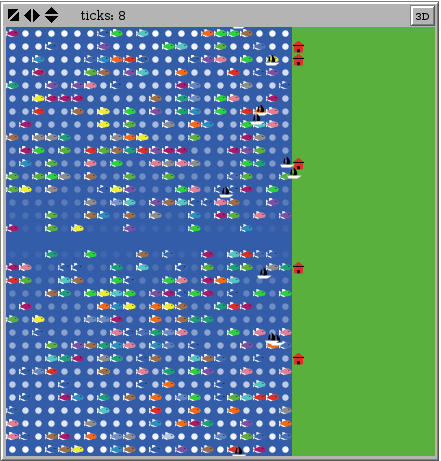
\includegraphics[scale=0.4]{img/espace.png}
		\end{center}
	\end{frame}
	
	\begin{frame}[c]{IODA}
			Méthode de modélisation à partir de laquelle a été créé une extension Netlogo - par Sébastien Picault et Philippe Mathieu de l'équipe SMAC (CRIStAL).
			\vfill
			\pause
			Buts:
			\begin{itemize}
			\item{simplifier un maximum le design et la réutilisation de simulations individu-centré,}
			\item{expliciter la matrice d'interactions et définir "proprement" les interactions.}
			\end{itemize}
			\vfill
			\url{http://www.lifl.fr/SMAC/projects/ioda/ioda_for_netlogo/}
	\end{frame}
	
	\begin{frame}[c]{IODA}{Principes de IODA}
			Principes de IODA:
			\begin{enumerate}
				\item{une entité est un agent,}
				\item{tout comportement est représenté par une interaction, composée d'un déclencheur optionnel (\textit{TRIGGER}), d'une condition (\textit{CONDITION}) ainsi que d'une action (\textit{ACTION}),}
				\item{ces interactions sont affectées à des familles d'agents, exécutées par un \textbf{moteur générique}.}
			\end{enumerate}
			\newline
			\color{red}{C'est le moteur qui détermine quelles interactions peuvent avoir lieu lors d'un pas de temps.}
	\end{frame}
	
	\begin{frame}[c]{IODA}{Fonctionnement du moteur générique IODA}
		Pour un pas de temps:
		\begin{enumerate}
			\item{les interactions de mises à jour (\textit{UPDATE}) réalisables sont exécutées par chaque agent donné,}
			\item{puis chaque agent susceptible d'agir sur les autres choisit une interaction de la façon suivante:
			\begin{enumerate}
				\item{perçoit ses voisins (subissant les actions des autres agents),}
				\item{filtre les cibles d'interactions qu'il peut effectuer,}
				\item{évalue les déclencheurs et conditions de ces interactions,}
				\item{sélectionne une des interactions réalisables (de priorité maximale),}
				\item{exécute les actions correspondantes, présentes dans la déclaration de l'interaction.}
			\end{enumerate}
			}
		\end{enumerate}
	\end{frame}
	
	\begin{frame}[c]{IODA}{Exemple}
		\begin{center}
			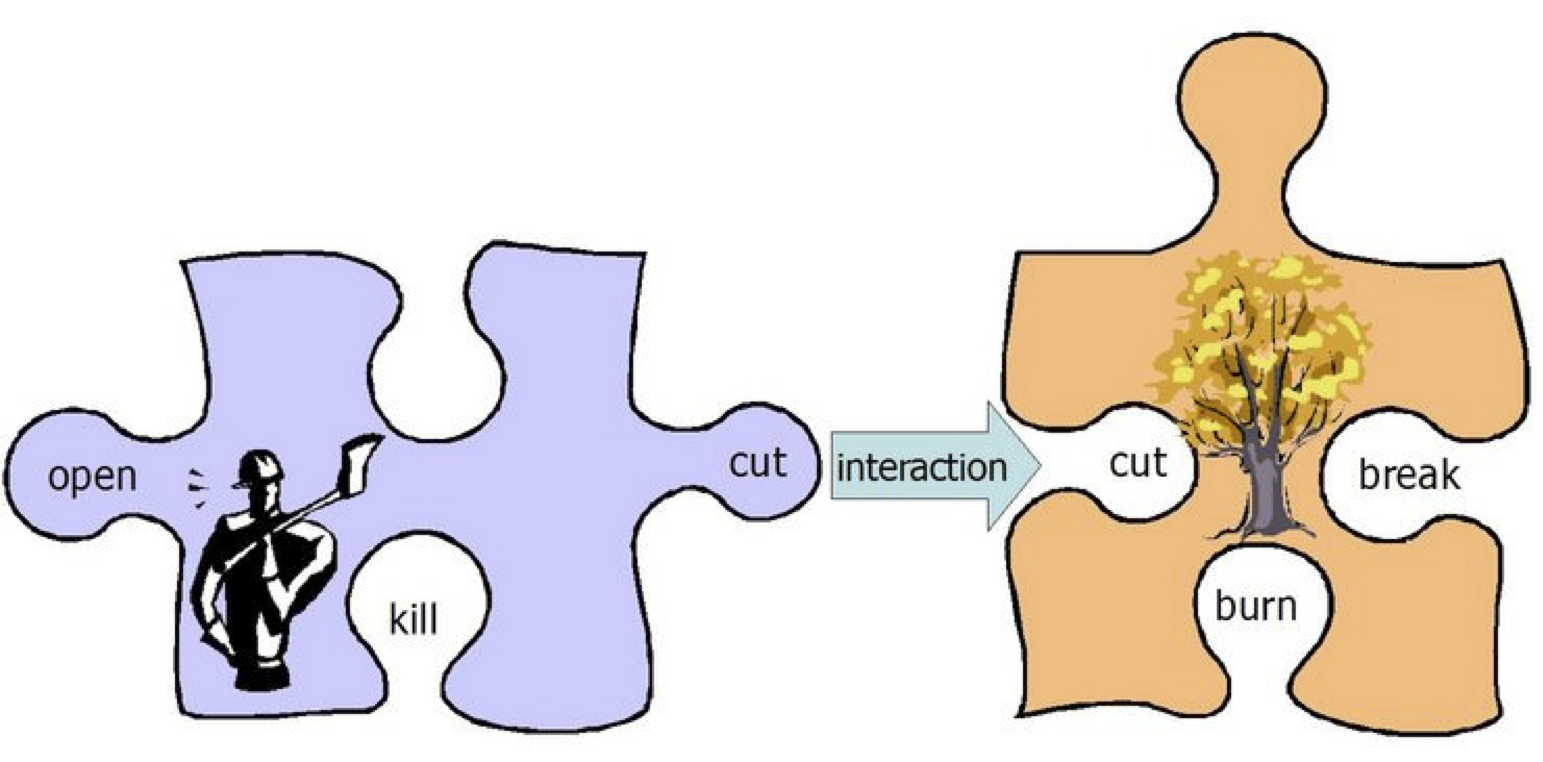
\includegraphics[scale=0.4]{img/moteur_ioda_explications.png}
		\end{center}
	\end{frame}
	
	\begin{frame}[c]{IODA}{Exemple}
		\begin{figure}[htbp]
		\makebox[\textwidth]{\hrulefill}{
		\small
		\verbatiminput{img/ioda_ex.txt}
		\normalsize}
		\end{figure}
	\end{frame}
	
	\section{La modélisation}
	
	\begin{frame}[c]{Modélisation}
		\begin{center}
			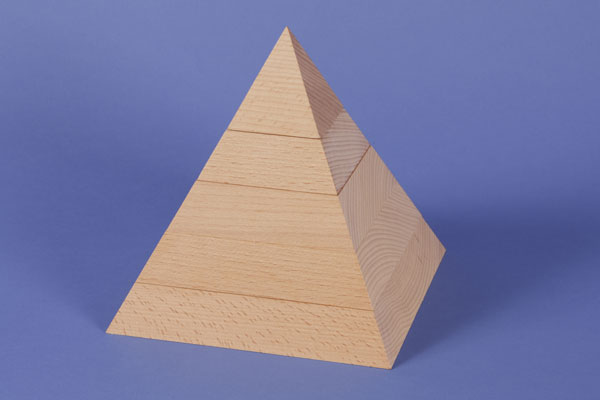
\includegraphics[scale=0.33]{img/pyramide.jpeg}
		\end{center}
		\only<2>{
		\begin{center}
		"Oh non, il est devenu complètement fou!"
		\end{center}
		}
		\only<3>{
		\begin{center}
		Modélisation empirique et incrémentale!!!
		\end{center}
		}
	\end{frame}
	
	\begin{frame}[c]{Modélisation}
			Découpage de la modélisation en 4 parties:
			\begin{itemize}
			\item{la modélisation d'une base,}
			\item{l'ajout de la chaîne alimentaire,}
			\item{l'expérimentation,}
			\item{l'ajout de l'activité concernant la pêche.}
			\end{itemize}
	\end{frame}
	
	\subsection{Un système simple}
	
	\begin{frame}[c]{Modélisation}
		\textbf{Idée}: modélisation d'un système proie/prédateur simple:
			\begin{itemize}
			\item{un agent proie: le plancton,}
			\item{un agent prédateur: les sardines.}
			\end{itemize}
		\vfill
		\pause
		\textbf{Besoins:} implémentation des agents et des interactions.
	\end{frame}
	
	\begin{frame}[c]{Modélisation}{Implémentation des premiers agents}
			Des caractéristiques propres, pour chaque agent:
			\begin{itemize}
			\item{\textbf{une biomasse},}
			\item{un nombre maximal de stock de nourriture (peut être égal à 0),}
			\item{zéro, une ou plusieurs cible(s),}
			\item{une biomasse cible (ce dont il a besoin pour [sur]vivre),}
			\item{une stratégie de migration,}
			\item{etc...}
			\end{itemize}
	\end{frame}
	
	\begin{frame}[c]{Modélisation}{Implémentation des premiers agents}
		Interactions définies dans la \textbf{matrice d'interactions}, et implémentées dans le \textbf{fichier d'interactions}. 
	\end{frame}
	
	\begin{frame}[c]{Modélisation}{Exemple}
		\begin{figure}[htbp]
		\makebox[\textwidth]{\hrulefill}{
		\small
		\verbatiminput{img/matrix_agents_ex.txt}
		\normalsize}
		\end{figure}
		\pause
		"L'agent \textit{sardines} va adopter pour le \textit{tick} \textbf{x} le comportement \textit{Eat} avec une priorité de 80, sur un agent \textit{food} à distance 0.5 de lui."
	\end{frame}
	
	\begin{frame}{Modélisation}{Exemple}
		\begin{figure}[htbp]
		\makebox[\textwidth]{\hrulefill}{
		\small
		\verbatiminput{img/matrix_ex.txt}
		\normalsize}
		\end{figure}
	\end{frame}
	
	\begin{frame}{Modélisation}{Exemple}
		\begin{figure}[htbp]
		\makebox[\textwidth]{\hrulefill}{
		\small
		\verbatiminput{img/ex_code.txt}
		\normalsize}
		\end{figure}
	\end{frame}
	
	\begin{frame}[c]{Modélisation}{Premiers résultats}
		Mini-objectifs:
		\begin{itemize}
			\item{modélisation et implémentation d'une base saine,}
			\item{modélisation d'un écosystème basique et général,}
			\item{devancement des problèmes liés à la suite de l'implémentation.}
		\end{itemize}
		\vfill
		\pause
		Partie longue et difficile!
	\end{frame}
	
	\subsection{La chaîne alimentaire}
        
        \begin{frame}{La chaîne alimentaire}{Modélisation}
          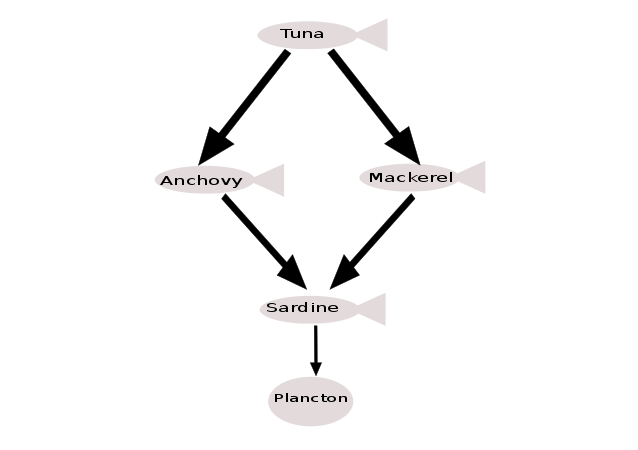
\includegraphics[height=0.9\textheight]{img/chaine_alimentaire.png}\centering
        \end{frame}
	
        
        \begin{frame}[c]{La chaîne alimentaire}{Nouvelles problématiques}
          De nouveaux défis:
          \begin{itemize}
          \item{nouvelles espèces,}
          \item{les mêmes interactions,}
          \item{nouvelles configurations.}
          \end{itemize}
          \vfill
        \end{frame}
        
        \begin{frame}{La chaîne alimentaire}{Les nouvelles configurations}
          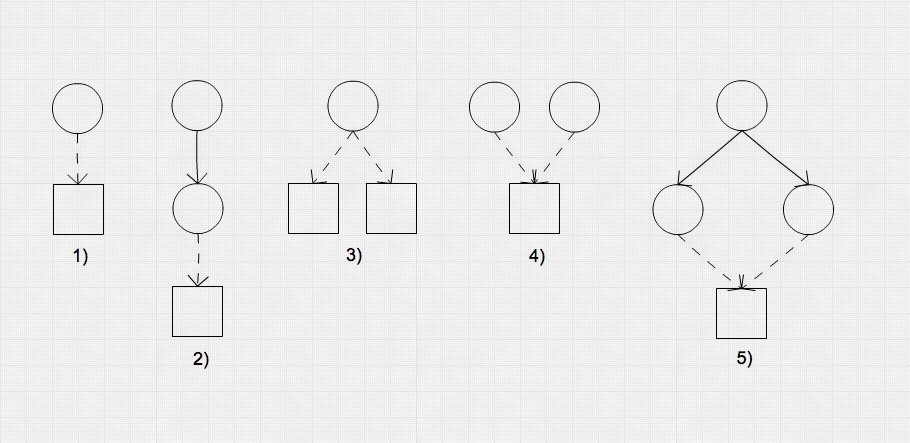
\includegraphics[width=\textwidth]{img/configuration.png}
        \end{frame}

        \begin{frame}[c]
          \begin{alertblock}{Problème}
            Modifications -> écosystème instable -> impossible de mesurer l'impact de la pêche.
          \end{alertblock}

          \pause
          
	  \begin{block}{Solution}
	    Une série d'expérimentations.
	  \end{block}
        \end{frame}
        
	\subsection{L'expérimentation}
	
        \begin{frame}[c]
          \frametitle{Evolution de la biomasse avant les expérimentations}
          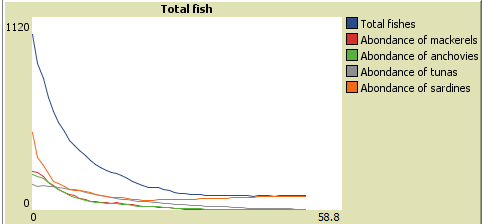
\includegraphics[width=\textwidth]{img/etape1.png}
        \end{frame}

        \begin{frame}[c]{Expérimentation}
          \begin{alertblock}{Problème}
            Enormément de paramètres entrent en jeu
            \begin{itemize}
            \item{stratégie de migration,}
            \item{consommation de nourriture,}
            \item{rapidité de reproduction,}
            \item{mortalité,}
            \item{stock de nourriture.}
            \end{itemize}
            Grand nombre d'expériences possibles!
          \end{alertblock}

          \pause

          \begin{block}{Solution}
            \begin{itemize}
            \item{Choix de 3 caractéristiques: consommation, reproduction et mortalité.}
            \item{Un protocole de recherche pour des recherches efficaces.}
            \end{itemize}
          \end{block}
        \end{frame}

        \begin{frame}{Expérimentation}{Méthodologie}
          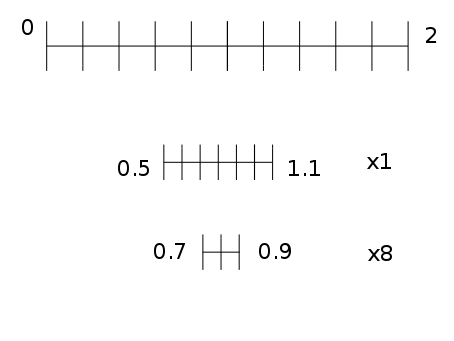
\includegraphics[width=\textwidth]{img/recherche.png}
        \end{frame}

        \begin{frame}[c]{Expérimentation}{Outils utilisés}
          \begin{center}
            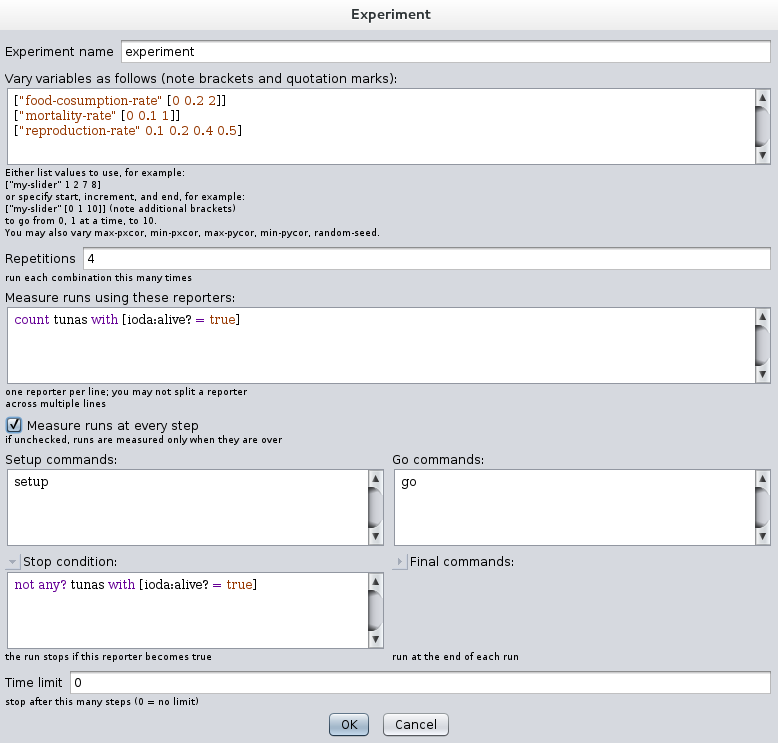
\includegraphics[height=0.8\textheight]{img/behaviorspace.png}
          \end{center}
        \end{frame}
        
        \begin{frame}{Expérimentation}{Évolution}
          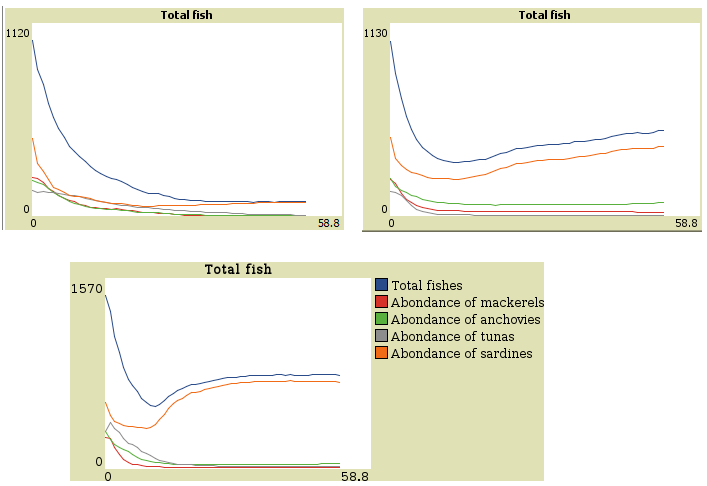
\includegraphics[width=0.9\textwidth]{img/evolution.png}
        \end{frame}
        
	\subsection{L'activité concernant la pêche}
	
        \begin{frame}{Intégration à la chaîne alimentaire}
          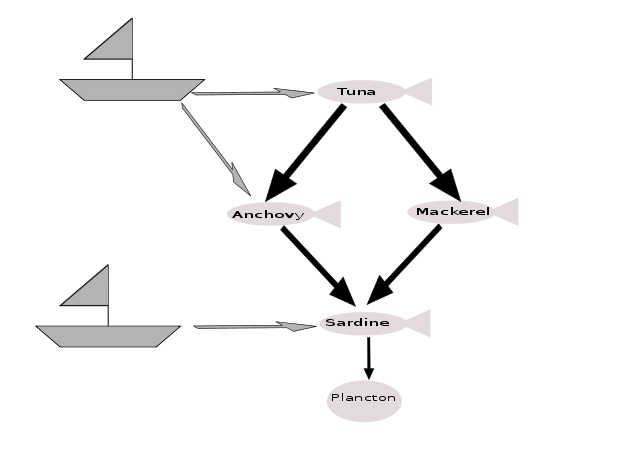
\includegraphics[height=0.9\textheight]{img/pecheur.png}
        \end{frame}        
        
        \begin{frame}[c]{L'activité concernant la pêche}{Problématique}
          Deux nouveaux agents nécessaires:
          \newline 
          \begin{itemize}
          \item{les ports:
            \begin{itemize}
            \item{possèdent un ou plusieurs bateaux,}
            \item{déterminent si les bateaux peuvent prendre la mer.}
            \end{itemize}
	  }
	  \item{les bateaux:
            \begin{itemize}
            \item{spécialisés,}
            \item{autonomes,}
            \item{stocker du poisson.}
	    \end{itemize}
	  }
          \end{itemize}
        \end{frame}

        \begin{frame}{L'activité concernant la pêche}{Nouvelles Interactions}
          \begin{figure}[htbp]
	    \makebox[\textwidth]{\hrulefill}{
	      \small
	      \verbatiminput{img/matrix_harbours_boats_matrix_ex.txt}
	      \normalsize}
	  \end{figure}
        \end{frame}
        
        \section{Résultats}
	
        \begin{frame}[c]{Résultats}{Serious-game}
          Différents éléments en jeu dans le serious-game:
          \begin{itemize}
          \item{aspect économique,}
          \item{aspect écosystème.}
          \end{itemize}
          Le joueur gère sa stratégie pour maximiser son score.
        \end{frame}
        
        \begin{frame}{Résultats}{Score}
          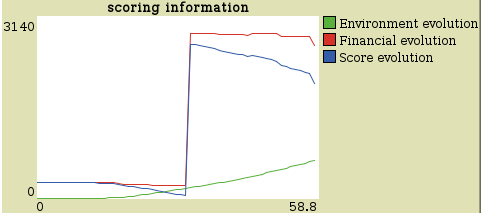
\includegraphics[width=\textwidth]{img/score.png}
        \end{frame}
        
        \begin{frame}{Résultats}{Au final...}
          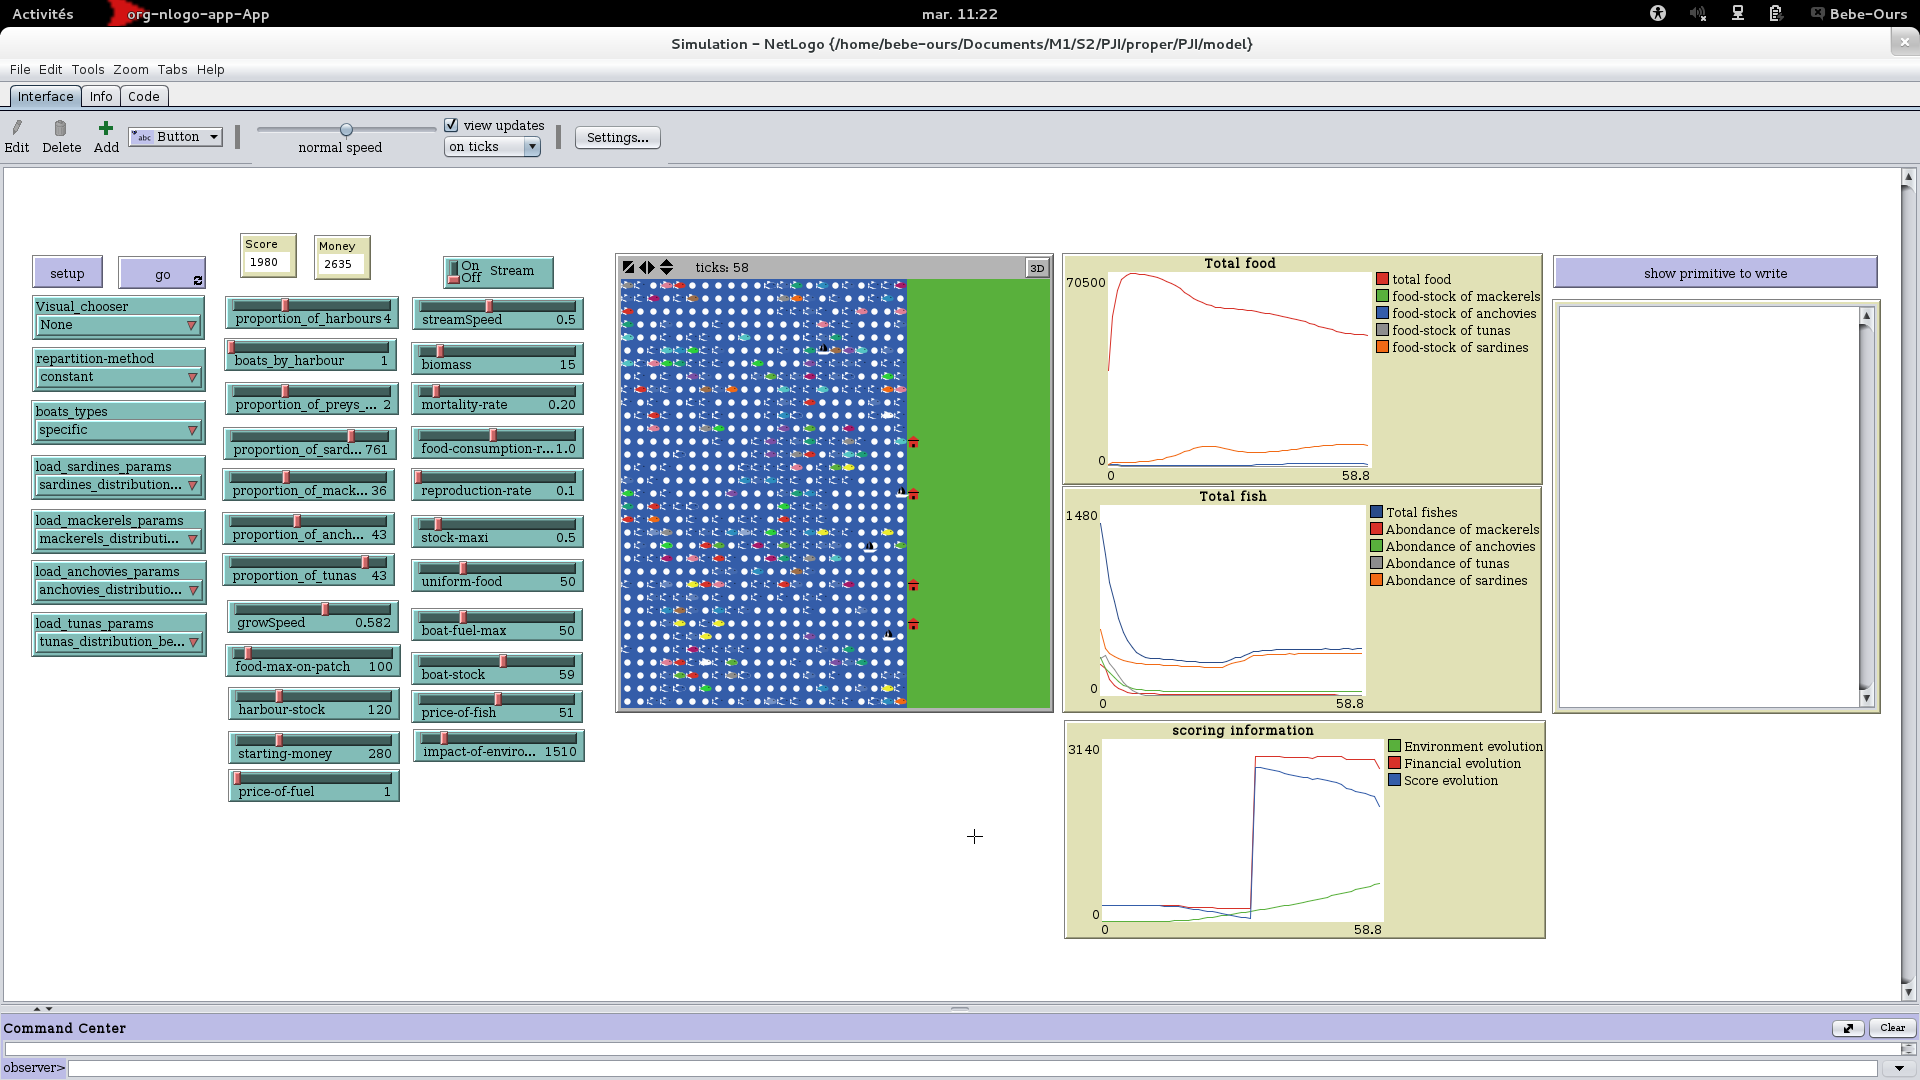
\includegraphics[width=\textwidth]{img/resultat.png}
        \end{frame}
        
	\section{Conclusion}
        
        \begin{frame}[c]{Conclusion}{Projet}
          Découverte de nouvelles technologies et méthodologies:
          \begin{itemize}
          \item{SMA et l'approche IODA,}
          \item{outils spécialisés dans la modélisation de SMA et la simulation,}
          \item{mise en place de stratégies d'expérimentation,}
          \item{développer un projet de manière incrémentale.}
          \end{itemize}
        \end{frame}
        
        \begin{frame}[c]{Conclusion}{Perspectives}
          Modèle:
          \begin{itemize}
          \item{integration de données réelles et d'éléments environnementaux,}
          \item{développer les différents aspects du serious-game,}
          \item{mesurer l'évaluation par les impacts indirects de la pêche sur l'écosystème,}
          \item{travailler la rejouabilité.}
          \end{itemize}
          Génie logiciel:
          \begin{itemize}
          \item{utilisation du moteur IODA en Python,}
          \item{utilisation du projet Netlogo en JavaScript.}
          \end{itemize}
          
        \end{frame}
        
        \begin{frame}[c]{Conclusion}{Personnel}
          \begin{itemize}
          \item{Compréhension des SMA.}
          \item{Travailler sur un sujet de recherche.}
          \item{Renforcer notre envie de suivre le Master MoCAD.}
          \end{itemize}
        \end{frame}
        
\end{document}
